\chapter{Hash tables}
\label{chapter:hashing}
When implementing an unordered dictionary, hashing is the most common tool
\footnote{Indeed, one of the many established meanings of the word ``hash''
	is ``unordered dictionary''.}
Hashing is a very old idea and the approaches to hashing are numerous. Hashing
techniques usually allow amortized constant-time \textsc{Find}, \textsc{Insert}
and \textsc{Delete} at the expense of disallowing \textsc{FindNext} and
\textsc{FindPrevious}. Certain schemes provide stronger than expected-time
bounds, like deterministic constant time for \textsc{Find}s in cuckoo hashing
(described in section \ref{sec:cuckoo}).

The idea of hashing is reducing the size of the large key universe
$\mathcal{U}$ to a smaller \emph{hash space} $H$ via a \emph{hashing function}
$h\mathop{:}\mathcal{U}\rightarrow H$.
In this chapter, let us denote the size of the hash space $M$.
\footnote{%
	No hashing schemes presented in this chapter are specific to external
	memory, so we do not need $M$ to denote the cache size in this chapter.
}
For a key $k$, we call $h(k)$ the \emph{hash} of $k$.

The size of the hash space is selected small enough to allow using hashes
of keys as indices in an array, which we call the \emph{hash table}.
The $i$-th element of the hash table may either be empty, or it may contain
a key-value pair $(k,v)$, where $h(k)=i$.

% TODO: figure

As long as all inserted keys have distinct hashes, hash tables are easy:
\textsc{Find}s, \textsc{Insert}s and \textsc{Delete}s all consist of just
hashing the key and performing one operation in the hash table -- it takes just
constant time, so also a constant number of memory transfers.
Unfortunately, if the set of stored keys is not known in advance,
some keys $k_1\neq k_2$ may have the same hash value.
This condition is called a \emph{collision}.

Specific collision resolution strategies differ between hashing approaches.

\section{Separate chaining}
\emph{Separate chaining} stores the set of all key-value pairs with
$h(k)=i$ in slot $i$. Let us call this set the \emph{collision chain} for hash
$i$, and denote its size $C_i$. The easiest solution is storing a pointer to
a linked list of colliding key-value pairs in the hash table. If there are no
collisions in an occupied slot, an easy and common optimization is storing
the only key-value pair directly in the hash table. However, following a longer
linked list is not cache-friendly.

If we use separate chaining, the costs of all hash table operations become
$\O(1)$ for slot lookup and $\O(|C_i|)$ for scanning the collision chain.
By picking a hash function that evenly distributes hashes among keys,
we can prove that the expected length of a collision chain is short.

To keep the expected chain length low, every time the hash table increases
or decreases in size by a constant factor, we rebuild it with a new $M$
picked to be $\Theta(N)$. The rebuild time is $\O(1)$ amortized per operation.

If we pick the hash function $h$ at random (i.e.,\ by independently randomly
assigning $h(k)$ for all $k\in\mathcal{U}$), we have $\forall i\in H,
k\in\mathcal{U}: \Pr[h(k)=i]=1/M$.
By linearity of expectation, we have $\E[C_i]=N/M$, which is
constant if we maintain $M=\O(N)$. Since the expected length of any chain
is constant, the expected time per operation is also constant.
The $N/M$ ratio is commonly called the \emph{load factor}.

However, storing a random hash function would require $|\mathcal{U}|\log M$
bits, which is too much: a typical hash table only stores a few keys from a
very large universe.
In practice, we pick a hash function from a certain smaller family according to
a formula with some variables chosen at random.
Given a family $\mathcal{H}$ of hashing functions, we call $\mathcal{H}$
\emph{universal} if $\Pr_{h\in \mathcal{H}}[h(x)=h(y)]=\O(\frac{1}{M})$ for any
$x, y\in\mathcal{U}$.
For any universal family of hash functions, the expected time per operation
is constant when using chaining.

A family $\mathcal{H}$ is $t$-independent if the hashes of $t$ distinct keys
$k_1,\ldots k_t$ are ``asymptotically independent'':
$$\forall k_1\neq\ldots \neq k_t\in K,
	h_1\ldots h_t\in H: \Pr_{h\in H}[h(k_1)=h_1\wedge \ldots \wedge
	h(k_t)=h_t]=\O(m^{-t})$$
2-independent hash function families are universal, but universal families
are not necessarily 2-independent.
Trivially, random hash functions are $k$-wise independent for any
$k\leq|\mathcal{U}|$.

% with cache of Omega(log n) totally random -> O(1) amortized per operation w.h.p.
% "pretty rare in practice", because hashing twice

Some common universal families of hash functions include:
\begin{itemize}
\item $h(k)=((a\cdot k)\bmod p)\bmod M$, where $p$ is a prime
	$\geq|\mathcal{U}|$ and $a\in\{0,\ldots p-1\}$ \cite{univ-classes}.
	The collision probability for this hash function is
	$\frac{\lfloor p/M\rfloor}{p-1}$, so it becomes less efficient
	if $M$ is close to $p$.
\item $(a\cdot k)\gg(\log u-\log m)$ for $M, |\mathcal{U}|$ powers of 2
	\cite{dietzfelbinger}.
	This hash function replaces modular arithmetic by bitwise shifts,
	which are faster on hardware.
\item \emph{Simple tabulation hashing} \cite{univ-classes}:
	% TODO: check citation
	interpret the key $x\in K$ as a vector
	of $c$~equal-size components $x_1,\ldots x_c$. Pick $c$ random hash
	functions $h_1,\ldots h_c$ mapping from key components $x_i$ to $H$.
	The hash of $x$ is computed by taking the bitwise XOR
	of hashes of all components $x_i$:
	$$h(x)=h_1(x_1)\oplus h_2(x_2)\oplus \ldots \oplus h_c(x_c)$$
	Simple tabulation hashes take time $\O(c)$ to compute in the general RAM
	model. Storing the $c$ individual hash functions needs space
	$\O(c\cdot |\mathcal{U}|^{1/c})$.  % TODO: approx u^\epsilon

	Simple tabulation hashing is 3-independent and not 4-independent,
	but a recent analysis in \cite{power-of-simple-tab} showed that
	it provides surprisingly good properties in some applications,
	some of which we will mention later.
\end{itemize}

While random hash functions combined with chaining give an expected $\O(1)$
time per operation, with high probability (i.e.,  $P=1-N^{-c}$ for an arbitrary
choice of $c$) there is at least one chain with at least $\O(\log N/\log\log N)$
items. The high-probability worst-case bound on operation time also applies
to hash functions with a high independence ($\O(\log N/\log\log N)$)
\cite{chernoff-hoeffding-bounds} and simple tabulation
hashing \cite{power-of-simple-tab}.

\section{Perfect hashing}
\emph{Perfect hashing} avoids the issue of collisions by picking a hashing
function that is collision-free for the given key set. If we fix the key set
$K$ in advance (i.e.,\ if we perform \emph{static hashing}), we can use
a variety of algorithms which produce a~collision-free hashing function at
the cost of some preprocessing time. If the hash function produces no empty
slots (i.e.,\ $M=N$), we call it \emph{minimal}.

For example, HDC (\textit{Hash, Displace and Compress},
\cite{hdc-hashing}) is a~randomized algorithm that can generate a~perfect
hash function in expected $\O(N)$ time. The hash function can be represented
using 1.98 bits per key for $M=1.01 N$, or more efficiently if we allow a~larger
$M$. All hash functions generated by HDC can be evaluated in constant time.
The algorithm can be generalized to build $k$-perfect hash functions, which
allow up to $k$ collisions per slot. The \textit{C Minimum Perfect
Hashing Library}, available at \url{http://cmph.sourceforge.net/}, implements
HDC along with several other minimum perfect hashing algorithms.

A dynamic version of perfect hashing, commonly referred to as \emph{FKS
hashing} after the initials of the authors, was developed in \cite{fks-hashing}.
FKS hashing takes worst-case $\O(1)$ time for queries (an improvement over
expected $\O(1)$ with chaining) and expected amortized $\O(1)$ for updates.

FKS hashing is two-level. The first-level hashing function $f$ partitions
the set of keys $K$ into $M$ buckets $B_1,\ldots B_M$. Denote their sizes as
$b_i$.
Every bucket is stored in a~separate hash table, mapping $B_i$ to an array
of size $\Theta(b_i^2)=\beta b_i^2$ via its private hash function $g_i$.
The constant $\beta$ will be picked later.
Each function $g_i$ is injective: buckets may contain no collisions.
% TODO: how can we store the fully random HF? why does it matter? maps from B_i?

If we pick the first-level hash function $f$ from a~universal family
$\mathcal{F}$, the expected total size of all buckets is linear, so an FKS
hash table takes expected linear space:
$$\E\left[\sum_{i=1}^N b_i^2\right]=
	\sum_{i=1}^N \sum_{j\in\{1,\ldots N\} \atop j\neq i}
	\Pr_{f\in\mathcal{F}}[f(k_i)=f(k_j)]=
	\O\left(N^2\cdot\frac{1}{M}\right)=\O(N)$$
We pick $f$ at random from $\mathcal{F}$ until we find one that will need at
most $\sum_{i=1}^N b_i=\alpha N$ space, where $\alpha$ is an appropriate
constant. Picking a~proper $\alpha$ yields expected $\O(N)$ time to pick $f$.

To select a~second-level hash function $g_i$, we pick one randomly from
a universal family $\mathcal{G}$ until we find one that gives no collisions
in $B_i$. By universality of~$g_i$, the expected number of collisions in $B_i$
is constant:
$$\E_{g_i\in\mathcal{G}}[\text{\# of collisions in }B_i]=
	{b_i\choose 2}\cdot\O\left(\frac{1}{b_i^2}\right)=\O(1)$$
By tuning the constant $\beta$, we can make the expected number of collisions
small (e.g., $\leq\frac{1}{2}$), so we can push the probability of having no
collisions above a~constant (e.g., $\geq\frac{1}{2}$). This ensures that for
every bucket, we will find an injective hash function in expected $\O(1)$
trials.

To \textsc{Find} a~key $k$, we simply compute $f(k)$ to get the right bucket,
and we look at position $g_{f(k)}(k)$ in the bucket, which takes deterministic
$\O(1)$ time.

Original static FKS hashing was extended to allow updates in
\cite{dyn-ph-bounds}.
We maintain $\O(N)$ buckets, and whenever $N$ increases or decreases by
a constant factor, we rebuild the whole FKS hash table in expected time
$\O(N)$, which amortizes to expected $\O(1)$ per update. Each bucket $B_i$
has $\O(b_i^2)$ slots. Whenever $b_i$ increases or decreases by a~constant
factor (e.g., 2), we resize the reservation by the constant factor's square
(e.g., 4).
The expected amortized time for \textsc{Insert} and \textsc{Delete} is $\O(1)$.
\cite{univ-class-of-hfns} enhances this to $\O(1)$ with high probability.

\section{Open addressing}
\label{sec:open-addressing}
When we attempt to \textsc{Insert} a~new pair with key $k$ into an occupied slot
$h(k)$, we can start trying out alternate slots $a(k,1), a(k,2), \ldots$
until we succeed in finding an empty slot. We call this approach \emph{open
addressing}. Examples of choices of $a(k,x)$ include:
\begin{itemize}
\item \emph{Linear probing}: $a(k,x)=(h(k)+x) \bmod M$
\item \emph{Quadratic probing}: $a(k,x)=(h(k)+x^2) \bmod M$
\item \emph{Double hashing}: $a(k,x)=[h(k)+x\cdot (1+h'(k))]\bmod M$, where
$h'$ is a~secondary hash function
\end{itemize}

When using this family of strategies, one also needs to slightly change
\textsc{Find} and \textsc{Delete}: \textsc{Find} must properly traverse
all possible locations that may contain the sought key, and \textsc{Delete}
and \textsc{Insert} must ensure that \textsc{Find} will know when to abort
the search.

To illustrate this point, consider linear hashing with $h(A)=h(C)=1$ and
$h(B)=2$. After inserting $A$ and $B$, slots 1 and 2 are occupied.
Inserting $C$ will skip slots 1 and 2, and $C$ will be inserted into slot 3.
When we try to look for $C$ later, we need to know that there are exactly 2 keys
that hash to 1, so we won't abort the search prematurely after only seeing
$A$ and $B$.

The ends of collision chains can be marked for example by explicitly maintaining
the lengths of collision chains in an array, or by marking the ends of chains
with a~bit flag.

All \textsc{Insert}s must traverse the entire collision chain to make sure
the inserted key is not in the hash table yet.
When we \textsc{Delete} a~key, we need to ensure that the collision chain
does not drift too far into alternative slots, so we traverse the entire
collision chain and move the last key-value pair in the chain to the slot
we deleted from.

By using \emph{lazy deletion}, one can avoid traversing the entire collision
chain in \textsc{Delete}s. Deleted elements are not replaced by elements from
the end of the chain, but they are instead just marked as deleted.
\textsc{Find} then skips over deleted elements and \textsc{Insert}s are allowed
to overwrite them.  \textsc{Find}s also ``execute'' the deletions by
overwriting the first encountered deleted slot by any pair from further down
the chain. An analysis of lazy deletions is presented in \cite{lazy-deletions}.

% TODO: document how exactly in our implementation
The reason why some implementations use quadratic probing and double hashing
over linear probing is that linear probing creates long chains when space is
tight. A~chain covering hash values $[i;j]$ forces any key hashing to this
interval to take $\O(j-i)$ time per operation and to extend the chain further.

However, linear probing performs well if we can avoid long chains: it has
much better locality of reference than quadratic or double hashing.
\cite{knuth-linear} showed that if $M=(1+\varepsilon) N$, then using a~random
hash function gives expected time $\O(1/\varepsilon^2)$ with linear probing.
\cite{linear-probing-ci} proved that 5-independent hash functions suffice
to get this bound, and \cite{linear-probing-constant} showed that
4-independence does not suffice.
\cite{power-of-simple-tab} gives a~proof that simple tabulation hashing,
which is only 3-independent and which can be implemented faster than usual
5-independent schemes, also achieves $\O(1/\varepsilon^2)$.

In section \ref{sec:hashing-results}, we present our measurements of the
performance of linear probing with simple tabulation hashing.

\section{Cuckoo hashing}
\label{sec:cuckoo}

A cuckoo hash table is composed of two hash tables $L$ and~$R$ of equal size
$M=(1+\varepsilon)\cdot N$.
Two separate hashing functions $h_\ell$ and $h_r$ are associated with
$L$~and~$R$.
All key-value pairs $(k,v)$ are stored either in $L$ at position $h_\ell(k)$,
or in $R$ at position $h_r(k)$.

The cuckoo hash table can also be visualized as a bipartite ``cuckoo graph'',
where partities are slots in $L$ and~$R$. Edges correspond to stored keys:
a stored key $k$ connects $h_\ell(k)$ in $L$ and~$h_r(k)$ in $R$. The assignment
of key-value pairs to slots in $L$ or $R$ forms a matching on the graph.

\textsc{Find}s take $\O(1)$ worst-case time: they compute $h_\ell(k)$ and $h_r(k)$
and look at the two indices in $L$~and~$R$. The two reads are independent and
can potentially be executed in parallel, especially on modern CPUs with
instruction reordering.

\textsc{Delete}s take $\O(1)$ time to find the deleted slot and to mark
it unused. Since the load factor of the cuckoo hash table needs to be kept
between two constants, \textsc{Delete}s end up taking $\O(1)$ amortized time
to account for rebuilds.

To \textsc{Insert} a new pair $(k,v)$, we examine slots $L[h_\ell(k)]$ and
$R[h_r(k)]$. If either slot is empty, $(k,v)$ is inserted there. Otherwise,
\textsc{Insert} tries to free up one of the slots, for example $L[h_\ell(k)]$.
If $L[h_\ell(k)]$ currently stores the key-value pair $(k_1,v_1)$, we attempt to
move it to $R[h_r(k_1)]$. If $R[h_r(k_1)]$ is occupied, we continue following
the path $k,k_1,k_2,\ldots$ until we either find an empty slot, or we find
a cycle.
The name ``cuckoo hashing'' refers to this procedure by analogy with
cuckoo chicks pushing eggs out of host birds' nests.

\begin{figure}
	\centering
	\begin{tikzpicture}[mpath/.style={font=\scriptsize,draw}]
	% Before
	\node (before-label) at (2,3.5) {Before};
	\matrix (left) [matrix of math nodes, row sep=-\pgflinewidth,
		column 2/.style={nodes={draw,rectangle,minimum width=2em, minimum height=2em}}]
	{L[0] & 4 \\ L[1] & 20 \\ L[2] & \times \\ L[3] & 40 \\ L[4] & \times \\
	L[5] & \times\\};

	\matrix (right) at (4,0) [matrix of math nodes, row sep=-\pgflinewidth,
		column 1/.style={nodes={rectangle,draw,minimum width=2em, minimum height=2em}}]
	{6 & R[0] \\ \times & R[1] \\ 30 & R[2] \\ \times & R[3] \\ \times & R[4] \\ 12 & R[5]\\};
	\path[mpath] (left-1-2.east) -- ([xshift=0.5cm]left-1-2.east) --
		node[above] {6}
		([xshift=-0.5cm]right-1-1.west) -- (right-1-1.west);
	\path[mpath] ([yshift=-0.2cm]left-1-2.east) -- ([xshift=0.5cm,yshift=-0.2cm]left-1-2.east) --
		node[above right] {4}
		([xshift=-0.5cm,yshift=0.2cm]right-3-1.west) -- ([yshift=0.2cm]right-3-1.west);
	\path[mpath] (left-2-2.east) -- ([xshift=0.5cm]left-2-2.east) --
		node[below left] {20}
		([xshift=-0.5cm]right-3-1.west) -- (right-3-1.west);
	\path[mpath] ([yshift=0.2cm]left-4-2.east) -- ([xshift=0.5cm,yshift=0.2cm]left-4-2.east) --
		node[below right] {30}
		([xshift=-0.5cm,yshift=-0.2cm]right-3-1.west) -- ([yshift=-0.2cm]right-3-1.west);
	\path[mpath] ([yshift=-0.2cm]left-4-2.east) -- ([xshift=0.5cm,yshift=-0.2cm]left-4-2.east) --
		node[below] {40}
		([yshift=-0.2cm,xshift=-0.5cm]right-4-1.west) -- ([yshift=-0.2cm]right-4-1.west);
	\path[mpath] (left-6-2.east) -- ([xshift=0.5cm]left-6-2.east) --
		node[below] {12}
		([xshift=-0.5cm]right-6-1.west) -- (right-6-1);

	% Obtaining free slot
	\node (obtaining-label) at (7.2,3.5) {Free up $L[h_\ell(10)]$};
	\matrix (l2) at (6.2,0) [matrix of math nodes, row sep=-\pgflinewidth,
		column 1/.style={nodes={draw,rectangle,minimum width=2em, minimum height=2em}}]
		{4 \\ 20 \\ \times \\ 40 \\ \times \\ \times\\};

	\matrix (r2) at (8.2,0) [matrix of math nodes, row sep=-\pgflinewidth,
		column 1/.style={nodes={rectangle,draw,minimum width=2em, minimum height=2em}}]
	{6 \\ \times \\ 30 \\ \times \\ \times \\ 12 \\};

	\path[->,mpath,thick,>=stealth] (l2-2-1) -- (r2-3-1);
	\path[->,mpath,thick,>=stealth] (r2-3-1) -- (l2-4-1);
	\path[->,mpath,thick,>=stealth] (l2-4-1) -- (r2-4-1);

	% After
	\node (after-label) at (11.35,3.5) {After};
	\matrix (l3) at (10.1,0) [matrix of math nodes, row sep=-\pgflinewidth,
		column 1/.style={nodes={draw,rectangle,minimum width=2em, minimum height=2em}}]
	{4 \\ 10 \\ \times \\ 30 \\ \times \\ \times\\};

	\matrix (r3) at (12.6,0) [matrix of math nodes, row sep=-\pgflinewidth,
		column 1/.style={nodes={rectangle,draw,minimum width=2em, minimum height=2em}}]
	{6 \\ \times \\ 20 \\ 40 \\ \times \\ 12 \\};
	\path[mpath] (l3-1-1.east) -- ([xshift=0.5cm]l3-1-1.east) --
		node[above] {6}
		([xshift=-0.5cm]r3-1-1.west) -- (r3-1-1.west);
	\path[mpath] ([yshift=-0.2cm]l3-1-1.east) --
	([xshift=0.5cm,yshift=-0.2cm]l3-1-1.east) --
		node[above right] {4}
		([xshift=-0.5cm,yshift=0.2cm]r3-3-1.west) -- ([yshift=0.2cm]r3-3-1.west);
	\path[mpath] ([yshift=0.1cm]l3-2-1.east) -- ([yshift=0.1cm,xshift=0.55cm]l3-2-1.east) --
		([yshift=0.1cm,xshift=-0.5cm]r3-3-1.west) -- ([yshift=0.1cm]r3-3-1.west);
	\path[mpath] (l3-2-1.east) -- ([xshift=0.5cm]l3-2-1.east) --
		node[xshift=-0.3cm,below] {10, 20}
		([xshift=-0.5cm]r3-3-1.west) -- (r3-3-1.west);
	\path[mpath] ([yshift=0.2cm]l3-4-1.east) --
	([xshift=0.5cm,yshift=0.2cm]l3-4-1.east) --
		node[below right] {30}
		([xshift=-0.5cm,yshift=-0.2cm]r3-3-1.west) -- ([yshift=-0.2cm]r3-3-1.west);
	\path[mpath] ([yshift=-0.2cm]l3-4-1.east) --
	([xshift=0.5cm,yshift=-0.2cm]l3-4-1.east) --
		node[below] {40}
		([yshift=-0.2cm,xshift=-0.5cm]r3-4-1.west) -- ([yshift=-0.2cm]r3-4-1.west);
	\path[mpath] (l3-6-1.east) -- ([xshift=0.5cm]l3-6-1.east) --
		node[below] {12}
		([xshift=-0.5cm]r3-6-1.west) -- (r3-6-1);
	\end{tikzpicture}

	\textsc{Insert}(10); $h_\ell(10)=1$, $h_r(10)=2$

	\caption{Inserting into a cuckoo hash table}
\end{figure}

If we find a cycle both on the path from $L[h_\ell(k)]$ and on the path from
$R[h_r(k)]$ (we can follow both at the same time), the cuckoo graph with
the added edge $(h_\ell(k),h_r(k))$ has no matching. To assign key-value pairs
to slots, we pick new hashing functions $h_\ell$ and $h_r$ and we rebuild
the entire structure.

To guarantee good performance, cuckoo hashing requires good randomness
properties of the hashing functions.
With $\Theta(\log N)$-independent hash functions, \textsc{Insert}s take
expected amortized time $\O(1)$ and the failure probability (i.e.,\ the
probability that an \textsc{Insert} will force a full rebuild) is
$\O(1/N)$ \cite{cuckoo-hashing}.
6-independence is not enough: some 6-independent hash functions lead to a
failure probability of $\O(1-\frac{1}{N})$ \cite{cuckoo-hashing-indep-bounds}.
The build failure probability when using simple tabulation hashing is
$\O(N^{1/3})$. \cite{power-of-simple-tab} demonstrates that storing all keys
$(a,b,c)$, where $a,b,c\in[N^{1/3}]$, is a degenerate case with
$\Omega(N^{1/3})$ build failure probability.

\begin{figure}
	\centering
	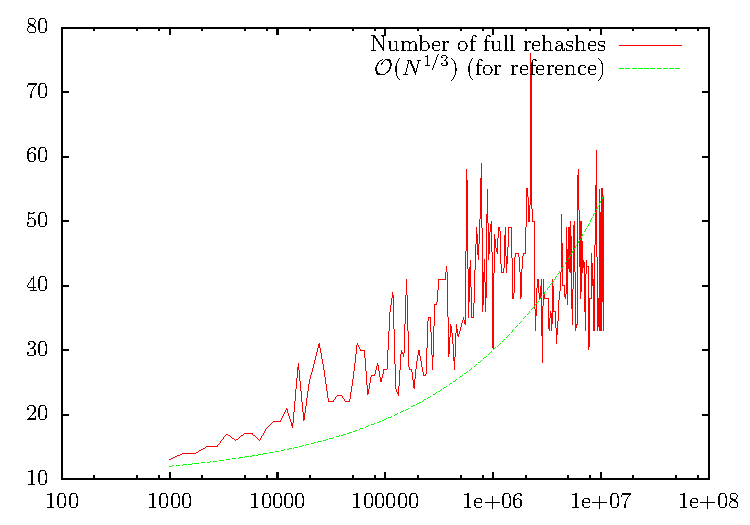
\includegraphics[width=0.7\textwidth]{img/cuckoo/results}
	\caption{Degenerate behavior of cuckoo hashing
		with simple tabulation ($\O(N^{1/3})$ rebuilds)
		as measured by our test program.}
\end{figure}

Examples of $\Theta(\log N)$-independent hashing schemes include:
\begin{itemize}
\item	For any $k$, a $k$-independent hash function family is \cite{new-hash-fns}:
	$$h(x)=\left(\sum_{i=0}^{k-1} a_i x^i \bmod p\right) \bmod M$$
	In this equation, $p$ is a prime greater than $|\mathcal{U}|$
	and all $a_i$ are chosen at random from $\Z_p$.
	This hash function family is considered slow due to needing
	$\Theta(\log N)$ time and using integer division by $p$.\footnote{%
		% TODO: This footnote looks like "p^2".
		As \cite{univ-classes} points out, using Mersenne primes
		(i.e.,\ $2^i-1$ for some $i$) enables a faster implementation of
		the modulo operation. On 64-bit keys, we could use $p=2^{89}-1$.
		It might not be possible to generalize this approach, because
		the question whether there are infinitely many Mersenne primes
		remains open.
	}
	Evaluation of this hash function takes $\O(k)$ steps on the RAM.
\item \cite{tab-based-4uni-hashing} presents a $k$-universal scheme that splits
	$x$ into $c$ components (as in simple tabulation hashing),
	expands $x$ into a \emph{derived key} $z$ of $\O(ck)$ components,
	and then applies simple tabulation hashing to $z$:
	$h(x)=\bigoplus h_i(z_i)$.
	When applied in our setting, where $c$ is fixed and $k=\O(\log N)$,
	the scheme takes time $\O(k)$ to evaluate.
	According to the authors, the scheme also has very competitive speed.
\item In order to outperform B-trees on the RAM, we would like to use a hashing
	function which evaluates faster than $\log N$. A scheme from
	\cite{univ-ext-random} needs only $\O(1)$ time to evaluate. Unfortunately,
	constructing a hash function by this scheme has high constant
	factors, so it is not very practical \cite{pagh-phd}.
\end{itemize}

% Both schemes need $\O(N^\epsilon)$ space to store the function.
% Drawback: large precomputed tables. CW-trick just requires $a_0,\ldots a_k-1$

For simplicity, our implementation of cuckoo hashing uses simple tabulation
hashing. As shown in section \ref{sec:hashing-results}, \textsc{Insert}s were
significantly slower than with linear probing. Our work could be extended by
trying more sophisticated and more independent hash functions.

\section{Extensions of hashing}
Several methods have been developed for maintaining hash tables in an external
memory setting without expensive rehashing. Some are presented in chapter 9
of \cite{em-ads}.

In \cite{kirsch2009more}, cuckoo hash tables are extended with a small
constant-sized \emph{stash} (e.g., 3 or 4 items), which lowers the probability
of build failures and enhances performance (both theoretically and practically).

Cuckoo hashing can be generalized to more than two subtables.
The \textsc{Insert} procedure then performs slot eviction via a random walk.
According to \cite{open-questions-cuckoo}, experiments suggest that cuckoo
hash tables with more functions may be significantly more effective than simple
cuckoo hashing on high load factors. For example, 3 subtables perform well
with loads up to 91\%. However, more subtables would lead to more potential
cache misses in \textsc{Find} on large hash tables.
